\documentclass[../thesis.tex]{subfiles}

\begin{document}
\chapter{Methods}
Figure \ref{fig:hc-approach} pictorially summarizes how we propose to solve the
hierarchical classification problem. It can be broken down into three major
areas: transforming the data into a meaningful feature space, grouping the
labels to form the label hierarchy, and using the label hierarchy to fit an HC.
\begin{figure}
    \centering
    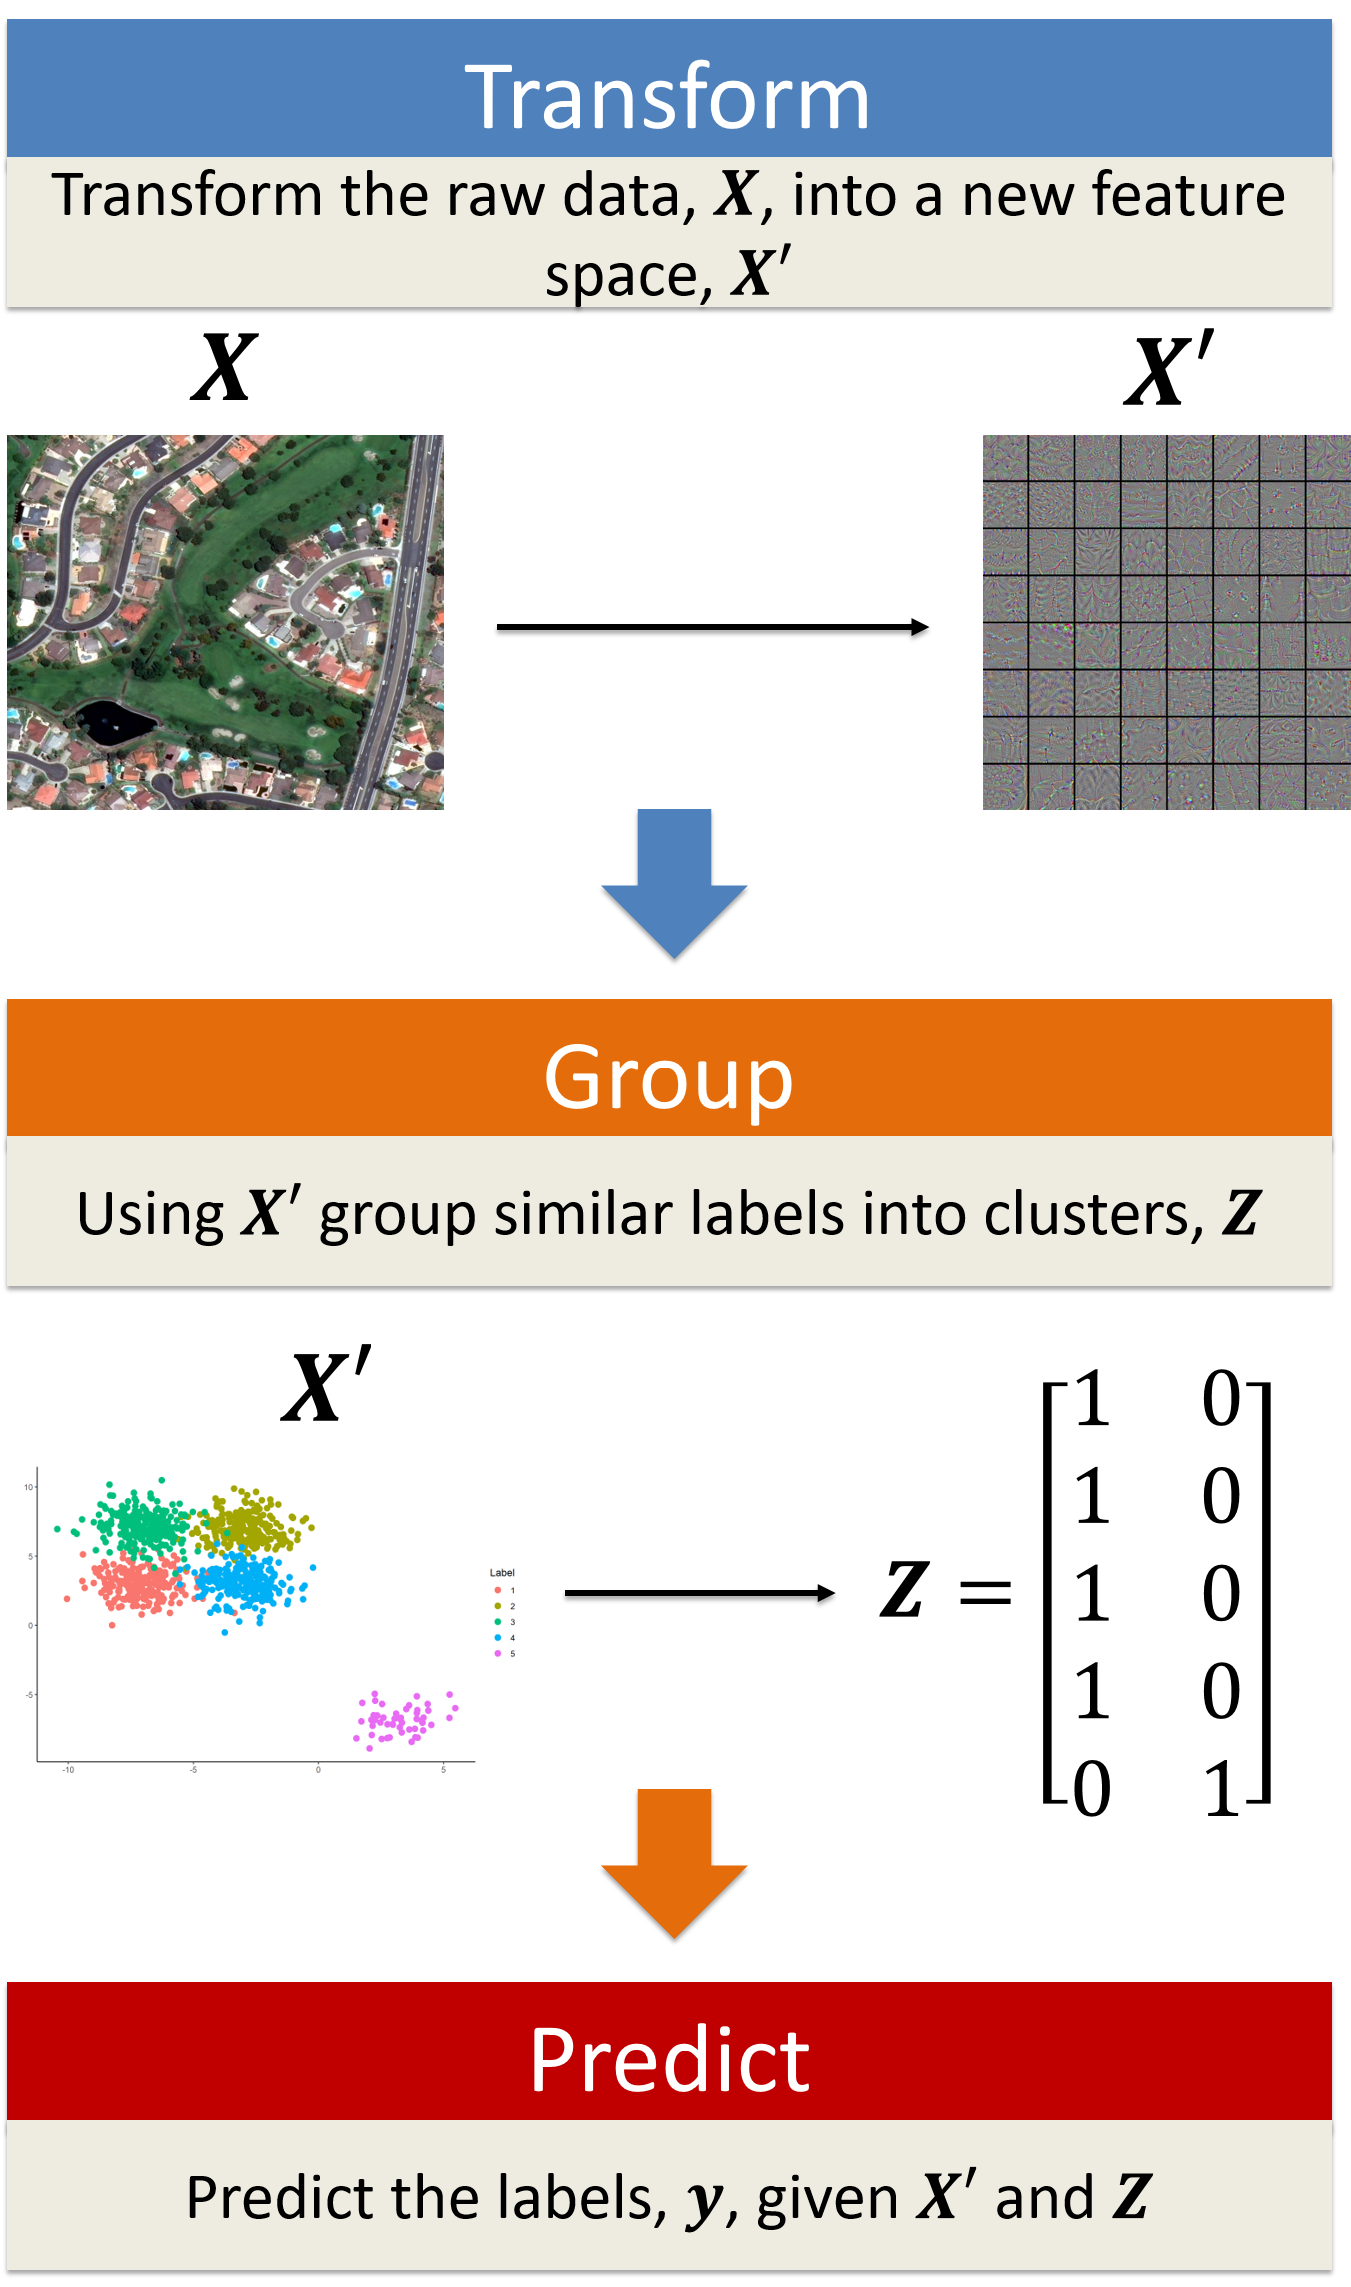
\includegraphics[width=.9\linewidth]{images/approach.pdf}
    \caption[Hierarchical Classification Approach]{This summarizes the three
    steps that need to be taken to solve the hierarchical classification
    problem. Our work primarily focuses on the ``grouping'' and ``prediction''
    stages, and we provide experimental context for the transformation
    components in Chapters 4 and 5.}
    \label{fig:hc-approach}
\end{figure}

In this chapter, we will highlight the major methodological contributions that
have been made in this thesis. The contributions fall into two major categories:
how to infer label groups and how to train and make predictions from an HC. We
will discuss how we transform the data in Chapters 4 and 5 because it can be
dependent upon the data type and structure, and we do not make any contributions
in this area. The methods we discuss in this chapter do however assume that the
data provided, $\mathcal{D} = (\mathbf{X}, \mathbf{y})$ is a meaningful
representation of the feature space.

\section{Label Hierarchy Inference}
In our research when working with HCs, we have focused on the case where the
label hierarchy is unknown potentially because there are too many labels for
this partition to be created by hand or asking an expert for a label grouping
would yield conflicting answers. Consequently, to employ an HC, the label
grouping must be inferred from the data. The standard way to do this, as
mentioned in Chapter 2, is to first trained a FC and then use spectral
clustering on a validation matrix to infer the label groups. This approach has
the advantage of tying the label hierarchy to classifier performance --
ultimately the most important metric -- however, this formulation requires that
we first train a flat classifier, which somewhat defeats the point of pursuing
this hierarchical approach and second to perform spectral clustering the user
must provide the number of meta-classes a-priori. We address the first primary
problem with spectral clustering with our two methods by employing k-means
clustering and a mixed-integer programming formulation, and we tackle both of
the problems when we propose a community detection based approach.

At the beginning of most of the label grouping methods we will discuss in this
chapter, we will provide a diagram that visually depicts the underlying approach
for this methodology. The purpose of these is to take what can be a quite
abstract topic and make the methodology more understandable.

\subsection{K-Means Clustering}
Figure \ref{fig:ex-kmeans} depicts the overall process we will employ to utilize
k-means clustering for providing label groupings: represent the labels as a
single point and then perform k-means clustering on this representation of the
data.
\begin{figure}
    \centering
    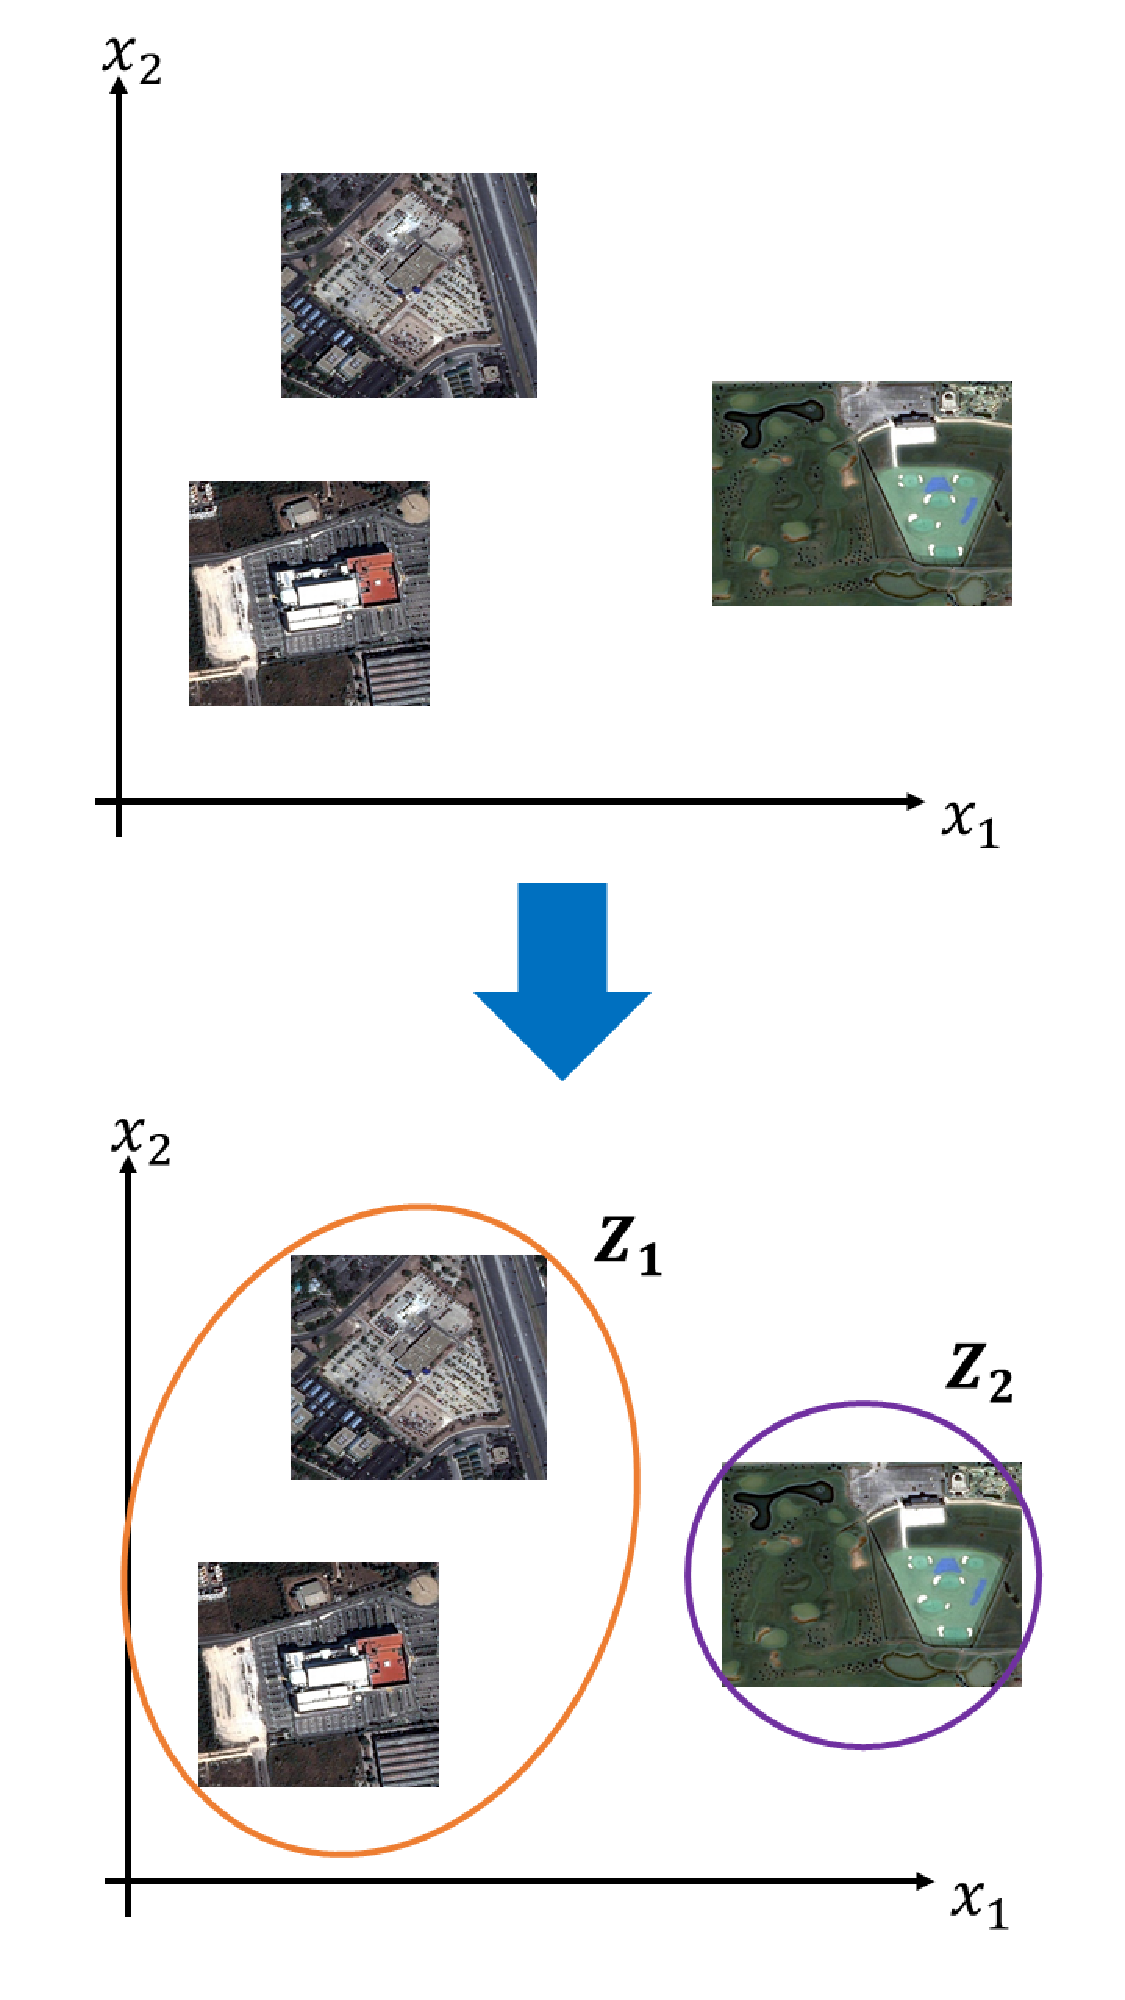
\includegraphics[width=.8\linewidth]{images/ex-kmeans.pdf}
    \caption[K-means Based Label Grouping]{This depicts an example of how the
    k-means algorithm is applied to group labels. In the first portion of the
    diagram, the three labels: shopping mall, car dealership, and golf course,
    are represented as a single point (in this case in two dimensions using
    principal component analysis for visualization purposes, but this is not
    necessary in general). Using the single points for the labels, the k-means
    clustering algorithm is then applied to generate the label groupings.}
    \label{fig:ex-kmeans}
\end{figure}

One of the major tasks of unsupervised machine learning is to find patterns in a
data matrix, $\mathbf{X}$, by finding ``clusters'' or groups of similar data
points. One of the most popular approaches to this task is an algorithm known as
k-means clustering \cite{jain2010data}. This algorithm was first proposed in
1967 by James MacQueen in his paper, \textit{Some Methods for Classification and
Analysis of Multivariate Observations} \cite{macqueen1967some}. Formulated as a
mixed-integer program (MIP), k-means clustering attempts to solve
\begin{mini}
	{\textbf{z}, \boldsymbol{\mu}}{\sum_{i=1}^C \sum_{j=1}^L z_{ij} \lVert
  \mathbf{v}_i - \boldsymbol{\mu}_j \rVert_2^2}
	{\label{eq:minlp}}{}
	\addConstraint{\sum_j z_{ij}}{= 1}{\quad \quad \forall i}
	\addConstraint{\sum_i z_{ij}}{\geq 1}{\quad \quad \forall j}
	\addConstraint{z_{ij}}{\in \{0, 1\}}{\quad \quad \forall i,j}
\end{mini}
However, (\ref{eq:minlp}) is a integer, non-convex opptimization problem --
traditionally a very difficult class of problems to solve to provable
optimiality \cite{burer2012non}. Instead of solving (\ref{eq:minlp}), the
k-means clustering finds a locally optimal partition of the data points in
$\mathbf{X}$. The standard algorithm was proposed by Stuart Lloyd in his paper,
\textit{Least Squares Quantization in PCM}, where he proposes k-means clustering
which has an ``assignment'' and ``update'' step \cite{lloyd1982least}. In the
assignment step, the algorithm places data points in certain clusters by
computing
\begin{equation}
    \label{eq:assign_step}
    S_i^t = \left \{ x_p : \lVert x_p - \mu_i^t \rVert_2^2 \leq \lVert x_p -
    \mu_j^t \rVert_2^2 \quad \forall j, 1 \leq j \leq k \right \}
\end{equation}
where $S_i^T$ and $\mu_i^t$ are the partition and centroid of the $i^{th}$
cluster at step $t$, respectively. In words what (\ref{eq:assign_step}) is
saying is that we will move a data point, $x_p$ into the $i^{th}$ cluster if the
distance from $x_p$ to $\mu_i^t$ is less than the distance of $x_p$ to the other
cluster centroids. In the event where the distances between two centroids is the
same, ties are broken arbitrarily. The second step of the k-means clustering
algorithm is the update step where the centroids are given new values after
various data points have been moved into different clusters. Mathematically this
step corresponds to
\begin{equation}
    \label{eq:update_step}
    \mu_i^{t+1} = \frac{1}{|S_i^t|} \sum_{x_j \in S_j^t} x_j.
\end{equation}
In short, (\ref{eq:update_step}) is stating that the centroid of cluster $i$ is
the average of the data points that have been moved into the partition during
the assignment step. The algorithm has converged if no points have changed
assignment; otherwise, the algorithm goes back to the assignment step. This
algorithm does not guarantee a globally optimal solution because it solves the
optimization problem proposed in (\ref{eq:minlp}) in a greedy fashion, but it is
very popular in practice due to its speed and simplicity
\cite{hartigan1979algorithm} \cite{jain2010data}.

Relating the k-means clustering algorithm to our problem, for our set-up we
assume that we have both a data matrix, $\mathbf{X} \in \R^{n \times p}$ and
labels $\mathbf{y} \in \{1, \ldots, C\}^n$; thus, this is by definition
\textit{not} an unsupervised machine learning problem. However, the goal is to
group similar labels with one another by using $\mathbf{X}$ and $\mathbf{y}$.
Thus this can indeed be viewed as an unsupervised problem.

Ultimately our goal is to infer some mapping matrix, $\mathbf{Z} \in \{0, 1\}^{C
\times k}$ where $k$ is provided and which follows the constraints provided in
(\ref{eq:minlp}). To this in a k-means clustering framework, we need to either
have some way of back-tracking to the target from the clustering or we need to
specifically encode a label as a single data point.

A first cut at this problem would be to perform k-means clustering on the data
matrix, $\mathbf{X}$, and then for each of the labels, determine the most common
cluster assignment and map that label to the particular grouping. This approach
is simple and easy to implement, but it does not guarantee that it will generate
a feasible solution. For example, suppose that the number of labels, $C = 3$,
and the number of meta-classes, $k=2$. \textbf{Insert diagram displaying extreme
case of this approach. This could be the circles dictating the three labels and
show how this can yield an infeasible solution.}

A better approach, and one that was first proposed by
\cite{vural2004hierarchical}, is to represent each label using its mean sample --
like (\ref{eq:kmeans_mean}). Doing this for all labels, $j = 1, \ldots, C$,
gives a matrix, $\mathbf{V} \in \R^{C \times p}$ where $\mathbf{v}_j$ represents
the mean point for the $j^{th}$ label. Consequently performing k-means
clustering on $\mathbf{V}$ will ensure that the resulting label map,
$\mathbf{Z}$ is feasible. In this thesis we employ this k-means based approach
as one of the techniques to infer a label hierarchy. This approach can
summarized succinctly in two steps
\begin{enumerate}
    \item Build the $\mathbf{V}$ matrix by computing (\ref{eq:kmeans_mean}) for
    all labels, $j = 1, \ldots, C$
    \item Perform k-means clustering on $\mathbf{V}$.
\end{enumerate}

The benefits of this approach is that it is simple and allows us to generate a
large number of candidate label hierarchies quickly. A simple question might be
though: how is what we are doing any different than what was proposed by Vural
and Dy in \cite{vural2004hierarchical}? The primary way we distinguish ourselves
from \cite{vural2004hierarchical} is that we do not force force $k=2$; instead
we treat the number of meta-classes as a hyper-parameter to be inferred using
cross-validation. The reason that \cite{vural2004hierarchical} set $k=2$ and
then recursively built the HC is that the authors were attempting to generate a
new binary classifier which can compute test predictions more quickly. This is
not our goal. Instead, we are interested in developing a HC which provides
superior performance relative to a flat classifier and the standard
spectral-clustering based approach to hierarchical classification. Second, if we
were to force $k=2$, this requires us to make $\left \lceil \log_2(C) \right
\rceil$ correct classifications to get the true label. The more correct
classifications that have to be made, the higher the probability that an error
will occur and thus propagate down the HC (this is also referred to as the
``routing problem'' and will be discussed later in this chapter).

\subsection{Mixed-Integer Programming Formulation}
One of the biggest weak points of the k-means clustering algorithm is that it
can stuck in bad local optima \cite{hartigan1979algorithm}. Common techniques to
avoid this issue are to provide better starting centroids (most commonly done
through the ``k-means++ algorithm'' \cite{arthur2007k}) and to perform a large
number of random restarts \cite{dick2014many}. However, an area that has shown
great research potential in recent years has been framing existing machine
learning problems and formulating them as MIPs.  For example, this has been done
with the best subset selection for a linear regression \cite{bertsimas2016best},
robust classification \cite{bertsimas2018robust}, and other common algorithms in
ML. The initial research results from this effort has shown that by framing
existing ML heuristics as MIPs, it possible to see significant out-of-sample
improvements. Using this as a starting point, we proposed to frame the k-means
clustering problem, as stated in (\ref{eq:minlp}) as a MIP to see if this could
yield outcomes.

However, the objective function in (\ref{eq:minlp}) cannot be linearized since
there is a quadratic term. Therefore instead of working with the $L_2$ norm, we
proposed to solve
\begin{mini!}
	{\textbf{z}, \boldsymbol{\mu}}{\sum_{i=1}^C \sum_{j=1}^L z_{ij}
  \left(\sum_{k=1}^p |v_{ik} - \mu_{jk}|\right)}
	{\label{eq:milp1}}{}
	\addConstraint{\sum_j z_{ij}}{= 1}{\quad \quad \forall i}
	\addConstraint{\sum_i z_{ij}}{\geq 1}{\quad \quad \forall j}
	\addConstraint{z_{ij}}{\in \{0, 1\}}{\quad \quad \forall i,j}
\end{mini!}
By introducing an absolute value in the objective function of (\ref{eq:milp1})
it is now possible to linearize the formulation by converting the absolute value
as well as the multiplication term in the objective.

To start since (\ref{eq:milp1}) is a minimization problem, the absolute value
component of the MIP can be reformulated to form a linear decision variable.
Specifically definite the auxiliary variable $\tau_{ijk} = |v_{ik} - \mu_{jk}$.
By definition of an absolute value, the following conditions must hold
\begin{align}
    v_{ik} - \mu_{jk} &\leq \tau_{ijk} \quad \quad \forall i, j, k \label{eq:abs1} \\
    \mu_{jk} - v_{ik} &\leq \tau_{ijk} \quad \quad \forall i, j, k \label{eq:abs2}
\end{align}
Clearly the constraints (\ref{eq:abs1}) and (\ref{eq:abs2}) can be quite
expensive given that we have three index sets to consider, but if the number of
features $k$ is kept to small size, then the problem does not become
unmanageable. Additionally, for notational simplicity, introduce the auxiliary
variable $\gamma_{ij} = \sum_k \tau_{ijk}$. Combining these constraints and
auxiliary variables we get the new formulation
\begin{mini!}
	{\textbf{z}, \boldsymbol{\mu}, \boldsymbol{\tau}, \boldsymbol{\gamma}}{\sum_{i, j} z_{ij} \gamma_{ij}}
	{\label{eq:milp2}}{}
	\addConstraint{\sum_j z_{ij}}{= 1}{\quad \quad \forall i}
	\addConstraint{\sum_i z_{ij}}{\geq 1}{\quad \quad \forall j}
	\addConstraint{v_{ik} - \mu_{jk}}{\leq \tau_{ijk}}{\quad \quad \forall i, j, k}
	\addConstraint{\mu_{jk} - v_{ik}}{\leq \tau_{ijk}}{\quad \quad \forall i, j, k}
	\addConstraint{\gamma_{ij}}{= \sum_k \tau_{ijk}}{\quad \quad \forall i, j}
	\addConstraint{z_{ij}}{\in \{0, 1\}}{\quad \quad \forall i,j}
\end{mini!}
However, (\ref{eq:milp2}) is still not a mixed-integer linear program (MILP)
because there is a non-linearity in the objective function: $z_{ij}
\gamma_{ij}$. This can be linearized by observing the following fact: by
definition
\begin{equation*}
    \gamma_{ij} = \sum_k \tau_{ijk} = \left(\sum_k |v_{ik} - \mu_{jk}|\right) \geq 0.
\end{equation*}
This implies that $\gamma_{ij}$ is lower-bounded by zero and has an upper bound
$M$ (we will discuss how we systematically go about finding this upper-bound
later in this section). Consequently, we introduce the new constraints and
auxiliary decision variables
\begin{align}
    \delta_{ij} &\leq Mz_{ij} \quad \quad \forall i, j \\
    \delta_{ij} &\leq \gamma_{ij} \quad \quad \forall i,j \\
    \delta_{ij} &\geq \gamma_{ij} - M(1-z_{ij}) \quad \quad \forall i, j \\
    \delta_{ij} &\geq 0 \quad \quad \forall i, j
\end{align}
Using these constraints we get the final, MILP formulation
\begin{mini!}
	{\textbf{z}, \boldsymbol{\mu}, \boldsymbol{\tau}, \boldsymbol{\gamma}, \boldsymbol{\delta}}{\sum_{i, j} \delta_{ij}}
	{\label{eq:milp3}}{}
	\addConstraint{\sum_j z_{ij}}{= 1}{\quad \quad \forall i}
	\addConstraint{\sum_i z_{ij}}{\geq 1}{\quad \quad \forall j}
	\addConstraint{v_{ik} - \mu_{jk}}{\leq \tau_{ijk}}{\quad \quad \forall i, j, k}
	\addConstraint{\mu_{jk} - v_{ik}}{\leq \tau_{ijk}}{\quad \quad \forall i, j, k}
	\addConstraint{\gamma_{ij}}{= \sum_k \tau_{ijk}}{\quad \quad \forall i, j}
	\addConstraint{\delta_{ij}}{\leq M z_{ij} \label{eq:big_m1}}{\quad \quad \forall i, j}
	\addConstraint{\delta_{ij}}{\leq \gamma_{ij}}{\quad \quad \forall i, j}
	\addConstraint{\delta_{ij}}{\geq \gamma_{ij} - M(1-z_{ij}) \label{eq:big_m2}}{\quad \quad \forall i, j}
	\addConstraint{\delta_{ij}}{\geq 0}{\quad \quad \forall i, j}
	\addConstraint{z_{ij}}{\in \{0, 1\}}{\quad \quad \forall i,j}
\end{mini!}
The MILP formulated in (\ref{eq:milp3}) can be quite large, particularly because
of the triple index constraint for $\tau_{ijk}$. However, given that $L \ll C$,
as long as the dimensionality of the data does not grow too rapidly,
(\ref{eq:milp3}) can be solved by employing a linear relaxation heuristic
discussed later in this section. However, before introducing the solution
heuristic we must first discuss how to systematically find values for the
big-$M$.

\subsubsection{Big $M$ Procedure}
We mentioned earlier that we can upper-bound the value for $\gamma_{ij}$ with
some value $M$, and it is important from a computational perspective that we are
able to find this value because we do not want to cut off solutions by having an
$M$ that is too small, but we also do not want to expand the search space
either. We will now discuss a procedure where we can systematically find a way
to upper-bound the value of $\gamma_{ij}$ such that we know we are not
eliminating any solutions while simultaneously having the tightest upper-bound
possible.

By definition $M$ corresponds to
\begin{equation*}
    M = \max \ \gamma_{ij} = \max \ \sum_k \tau_{ijk} = \max \
    \left(\sum_k |v_{ik} - \mu_{jk}|\right).
\end{equation*}
Formally, I claim:

\begin{theorem}
    It is sufficient to find the $\max \ \left(\sum_k |v_{ik} -
    \mu_{jk}|\right)$ when $j = 1$ because the value is the same for every $j
    \in \{1, \ldots, L\}$.
\end{theorem}

\begin{proof}
    Suppose we have some vector $\mathbf{v}_i = (v_{i1}, v_{i2}, \ldots,
    v_{ip})^T$ and let $L$ be the number of meta-classes. Let $M_{ij}$ be the
    solution to the constrained optimization problem
    \begin{maxi}
    	{\boldsymbol{\mu}}{\sum_k |v_{ik} - \mu_{jk}|}
    	{\label{eq:big_m}}{}
    	\addConstraint{\mu_{jk}}{\geq L_k}{\quad \quad \forall k}
    	\addConstraint{\mu_{jk}}{\leq U_k}{\quad \quad \forall k}
    \end{maxi}
    where $L_k$ and $U_k$ define the lower and upper bounds of the data which is
    inferred from $\mathbf{V}$. We know these constraints must exist because in
    the original problem of finding the centroids which \textit{minimize} the
    $L_1$ distance, clearly the algorithm would never select a point $\mu_{jk}$
    which was greater than $U_k$ or smaller than $L_k$. This is true because the
    objective value of (\ref{eq:milp1}) could be reduced by simply moving
    $\mu_{jk} = L_k$ if it was beyond the lower bound or $\mu_{jk} = U_k$ if it
    was greater than the upper bound.

    Using this fact, we see that the constraints in (\ref{eq:big_m}) hold
    regardless of the meta-class index. That is, for every $j \in \{1, \ldots,
    L\}$ $\boldsymbol{\mu}_j$ is subject to the same constraints. This implies
    that (\ref{eq:big_m}) is the same optimization problem regardless of the
    meta-class index which necessarily means that
    \begin{equation*}
        \boldsymbol{\mu}_1 = \boldsymbol{\mu}_2 = \cdots = \boldsymbol{\mu}_L.
    \end{equation*}
    Therefore since we defined $M_{ij}$ as the solution to (\ref{eq:big_m}) this
    means that
    \begin{equation*}
        M_{i1} = M_{i2} = \cdots = M_{iL}.
    \end{equation*}
    Thus we know that it is sufficient to solve the optimization problem for $j =
    1$ because $M_{ij}$ is the same for all $j$.
\end{proof}

Now that we have proved that the bound $M_{ij}$ is only dependent upon the given
label $i$ and not the meta-class, $j$, we need to propose a way to find $M_i$
for every $i \in \{1, \ldots, C\}$. To do this, we will show a simple
two-dimensional and show how we can easily infer what $M_i$ must be for a given
label.

Suppose we have a $\mathbf{V}$ matrix equal to
\begin{equation*}
    \mathbf{V} =
    \begin{bmatrix}
        2 & 3 \\
        2 & 2 \\
        3 & 2 \\
        5 & 1 \\
    \end{bmatrix}
\end{equation*}
and we are interested in finding $M_1$ -- the max possible value for
$\left(|v_{11} - \mu_{j1}| + |v_{12} - \mu_{j2}|\right)$. Using these values, we
get the plot shown in Figure \ref{fig:big-m-plot} where $L_k$ and $U_k$ define
the lower and upper bound for the $k^{th}$ dimension.
\begin{figure}
    \centering
    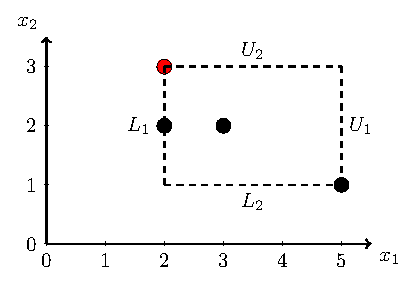
\includegraphics{images/big-m-plot.pdf}
    \caption[Big $M$ Inference Example]{This plot depicts a situation where
    there are four labels in two dimensions. Focusing specifically on the red
    label, the dashed lines depict the upper and lower bounds for the values of
    the data and the corresponding value for $M_1$ must exist on one of the four
    vertices of the rectangle as a consequence of minimizing an $L_1$ norm.}
    \label{fig:big-m-plot}
\end{figure}

In this instance, observe that $\mu_{j, 1} \in [2, 5]$ and $\mu_{j, 2} \in [1,
3]$. Since we are interested in maximizing the $L_1$ norm, it is sufficient to
greedily find the maximum value for each dimension to determine $\mu_{jk}^*$ and
then we can aggregate these value to compute $M_i$. Moreover, the maximum value
for any given $\mu_{jk}^*$ must occur at the boundaries of the feasible set.
This is true because one of the constraints in (\ref{eq:big_m}) must hold
tightly at optimality because otherwise we could increase the objective function
by making either the lower or upper bound constraint tight. Thus for the case of
solving $M_1$, observe that $v_1 = (3, 2)$ and thus for $\mu_{j1}$ we can either
select two or five and for $\mu_{j2}$ the options are one or three. Since we are
interested in computing the upper bound for a given label we can greedily solve
the optimization problems
\begin{equation*}
    m_{i1}^* = \underset{\{2, 5\}}{\text{max}} \ \left\{|2-2|, |2-5|\right\} = 3
\end{equation*}
and
\begin{equation*}
    m_{i2}^* = \underset{\{1, 3\}}{\text{max}} \ \left\{|3-1|, |3-3|\right\} = 2
\end{equation*}
where $m_{ik}^*$ is the maximal distance for the $k^{th}$ dimension for some
point for the $i^{th}$ label. We then can get the final upper-bound $M_i$ by
computing
\begin{equation}
    M_i = \sum_k m_{ik}^*.
\end{equation}

Ultimately the analysis we have conducted in this section allows us to write a
very simple algorithm to compute the upper bound for each of the labels in the
data set.
\begin{algorithm}
    \caption{Upper-Bound Algorithm}
    \label{alg:upperbound}
    \begin{algorithmic}[1]
        \Procedure{find bounds}{$\mathbf{V}$}
            \For{$k \in \{1, \ldots, p$\}} \Comment{Get the upper and lower
            bounds for every $k$}
                \State $L_k \gets$ min $\left\{v_{1k}, \ldots, v_{Ck}\right\}$
                \State $U_k \gets$ max $\left\{v_{1k}, \ldots, v_{Ck}\right\}$
            \EndFor
            \For{$i \in \{1, \ldots, C\}$} \Comment{Compute $M_i$ for every $i$}
                \For{$k \in \{1, \ldots, p$\}}
                    \State $m_{ik}^* \gets$ max $\left\{|v_{ik} - L_k|, |v_{ik}
                    - U_k|\right\}$
                \EndFor
                \State $M_i \gets \sum_k m_{ik}^*$
            \EndFor
            \State \textbf{return} $(M_1, \ldots, M_C)$
        \EndProcedure
    \end{algorithmic}
\end{algorithm}

Algorithm \ref{alg:upperbound} involves simply computing the upper and lower
bounds for every dimension and then using those bounds to infer the largest
possible value for a given label. We can therefore update the constraints
(\ref{eq:big_m1}) and (\ref{eq:big_m2}) to be
\begin{align}
    \delta_{ij} &\leq M_i z_{ij} \quad \forall i, j \\
    \delta_{ij} &\geq \gamma_{ij} - M_i(1-z_{ij}) \quad \forall i, j
\end{align}
where instead of having a singular upper bound $M$ (which would be $M =
\text{max} \left\{M_1, \ldots, M_C\right\}$), we instead can have a more refined
bound for each class. As a consequence of employing this trick, we decrease the
feasible region while maintaining the requirement that no feasible solutions be
removed from the polyhedron.

\subsubsection{Linear Relaxation}
Even though we employed a number of linearization tricks to conver the MINLP,
(\ref{eq:minlp}), into a MILP, oftentimes, (\ref{eq:milp3}), we still be quite
difficult to solve, particularly because of the triple index auxiliary variable,
$\tau_{ijk}$. This variable is dependent on both the number of classes and the
desired number of label groupings as well as the dimensionality of the feature
space which can be quite high. For example, the feature extract technique
employed throughout the experiments yields a vector which has $4000+$ features.
Therefore to be able to solve (\ref{eq:milp3}) in an appropriate amount of time,
we employ a linear relaxation trick to convert the problem from a MILP to a
standard linear program.

The only integer variables in the formulation are the values $z_{ij}$ which
denote whether the label $i$ has been placed in meta-class $j$. This is a binary
variable and thus can be relaxed to a new variable, $z_{ij}^\prime \in [0, 1]$.
However, since we are solving a LP approximation of the original MILP, we are
not guaranteed to generate feasible solutions to the original problem and thus
it is necessary to employ a conversion technique which will transform the LP
solution into a feasible solution for the MILP in the event that the resulting
partition matrix, $\mathbf{Z}$ does not yield all integer values. To develop
such a conversion, let us briefly return to the original, non-linear formulation
before we employed a number of linearization techniques. In (\ref{eq:minlp}) we
have two primary variables of interest: the meta-class matrix, $\mathbf{Z}$, and
the centroids of the label groupings: $\boldsymbol{\mu}$. Moreover, there are
only two relevant constraints; in words these are:
\begin{enumerate}
    \item Every label must be assigned to a meta-class
    \item Every meta-class must contain at least one label
\end{enumerate}
For the feasible solution technique we will introduce, only the first constraint
is necessary. Viewed differently, the constraints that $z_{ij} \in [0, 1]$ and
$\sum_j z_{ij} = 1$ define a discrete probability distribution. Recall that a
valid probability mass function for some random variable, $X$, has the following
properties \cite{blitzstein2014introduction}:
\begin{enumerate}
    \item $\mathbf{P}(X = x) \geq 0$ for all $x \in X$
    \item $\sum_{x \in X} p_X(x) = 1$.
\end{enumerate}
For the linear relaxation of the (\ref{eq:milp3}), a row of the label grouping
matrix, $\mathbf{z}_j$, can have non-negative mass for $L$ values of the vector,
of which no value can be greater than one and the sum of the $L$ items must
equal one. Thus, by definition a row of the partition matrix can be viewed as a
probability distribution. Consequently this suggests that we can employ a
sampling technique to generate feasible integer solutions. To make this
concrete, we will start with a small example and then provide the overall
algorithm.

Suppose that the linear relaxation for (\ref{eq:milp3}) for a problem with $C=3$
labels and $L=2$ meta-classes yielded the solution:
\begin{equation*}
    \mathbf{Z}^\prime =
    \begin{bmatrix}
        0.67 & 0.33 \\
        1 & 0 \\
        0.5 & 0.5
    \end{bmatrix}
\end{equation*}
To generate integer feasible solutions from $\mathbf{Z}^\prime$, from the first
row for instance, we could sample proportional to the ``distribution.''
Specifically, with probability $0.67$ we will place a one in the first column
and with probability $0.33$ a one is placed in the second column. This same
technique can be repeated for all of the other rows in $\mathbf{Z}^\prime$.
Consequently this will generate a feasible integer solution (assuming that all
of the columns have at least one entry in them). Moreover, this procedure can be
done many times generating hundreds of unique, feasible integer solutions. The
objective value of these solutions can then be computed and the one with the
lowest error value can be treated as the final solution to the problem. There
are further improvements that can be taken with this procedure (i.e., employing
a local search to further refine the partition matrix), but this is discussed
more in Chapter 6.

The algorithm detailing this sampling procedure is shown in Algorithm
\ref{alg:sampling-procedure}.
\begin{algorithm}
    \caption{Feasible Solution Generation}
    \label{alg:sampling-procedure}
    \begin{algorithmic}[1]
        \Procedure{Generate Solution}{$\mathbf{V}$, $n$}
            \State $\mathbf{Z}^\prime \gets$ Solution to linear relaxation of (\ref{eq:milp3})
            \State Define placeholder matrices $\{\mathbf{Z}^1, \ldots,
            \mathbf{Z}^n\}$ and placeholder objective values $\mathbf{s} =
            (\infty, \ldots, \infty)$
            \For{$i \in \{1, \ldots, n\}$}
                \For{$j \in \{1, \ldots, C\}$}
                    \State $l \gets $ Sample proportionally to $\mathbf{z}_j^\prime$
                    \State $Z^i_{jl} = 1$
                \EndFor
                \If{$\mathbf{Z}^i$ is not feasible} \Comment{Checking
                constraints in (\ref{eq:milp1})}
                    \State Discard $\mathbf{Z}^i$
                \Else{}
                    \State $\boldsymbol{\mu}^i \gets$ Infer from $\mathbf{V}$
                    and $\mathbf{Z}^i$
                    \State $\mathbf{s}_i \gets$ Compute objective using
                    $\mathbf{Z}^i$ and $\boldsymbol{\mu}^i$
                \EndIf
            \EndFor
            \State $m^* \gets \argmin \{s_1, \ldots, s_n \}$
            \State \textbf{return} $\mathbf{Z}^{m^*}$
        \EndProcedure
    \end{algorithmic}
\end{algorithm}

Using Algorithm \ref{alg:sampling-procedure}, we can generate feasible label
groupings in a computationally tractable manner.

\subsection{Community Detection}
Figure \ref{fig:ex-community-detection} depicts the process employed utilize
community detection algorithms to infer label partitions: represent the labels
as a graph using some similarity metric, and then use a community detection
algorithm.
\begin{figure}
    \centering
    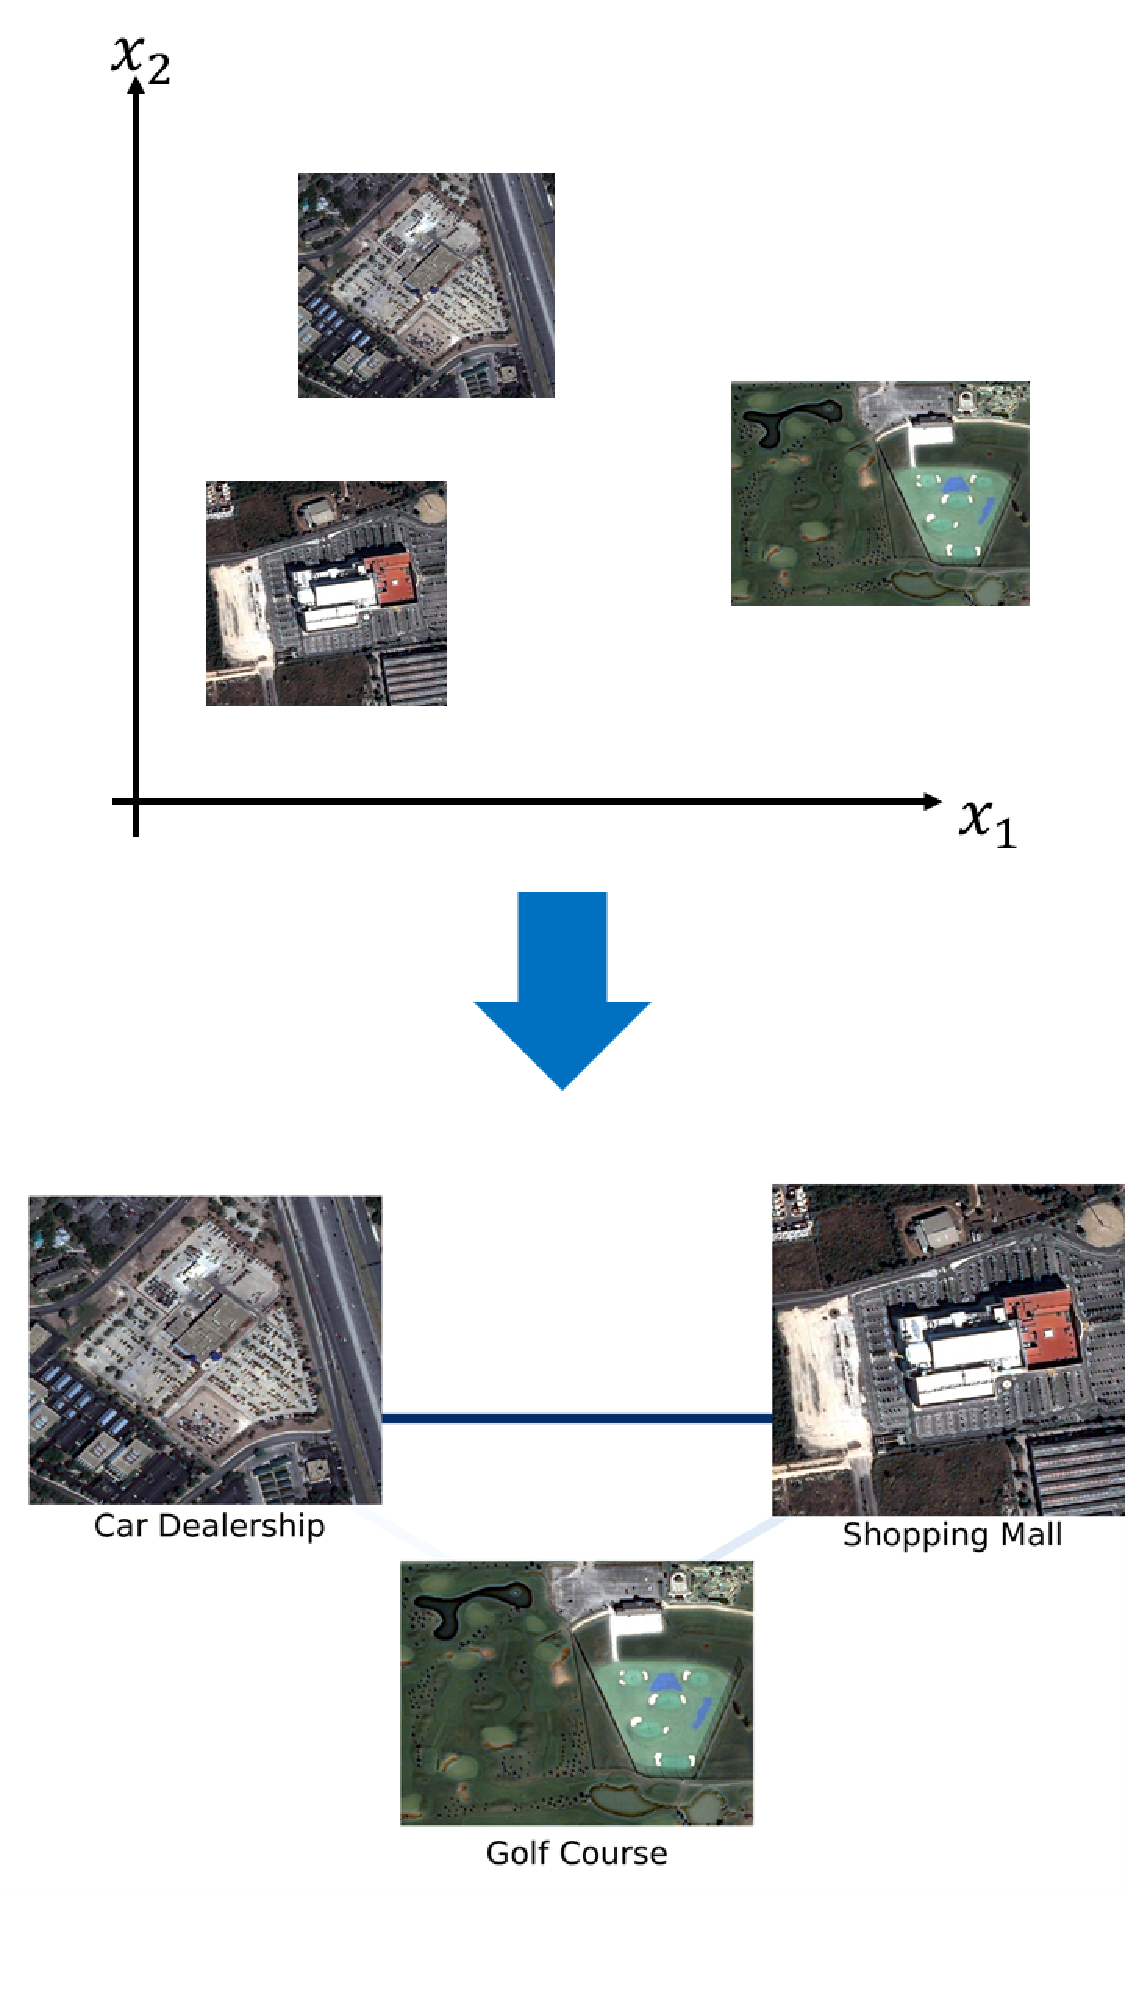
\includegraphics[width=.8\linewidth]{images/ex-community-detection.pdf}
    \caption[Community Detection Based Label Grouping]{This diagram the approach
    that we take to solve the label grouping problem using community detection.
    Like the k-means approach, we again represent the labels as single points.
    However, to employ a community detection algorithm we have to represent the
    labels as a graph. This is done by computing some similarity metric. The
    strength of the connection is denoted by the darkness of the edge in the
    figure}
    \label{fig:ex-community-detection}
\end{figure}

One of the major drawbacks of the employing either the k-means based approach or
the MILP is that the user must specify the number of meta-classes in the data
before using the algorithm. Consequently this requires the analyst to either
know approximately how many groups are contained in the data beforehand or to
treat this value as a hyper-parameter which inferred via cross-validation. The
second case is the more typical approach because oftentimes one might know a
reasonable range of values, but not the optimal number of label groupings.
However, what if we did not have to specify the number of meta-classes? What if
we had an algorithm that could infer this parameter automatically? This question
motivates our third approach to the label grouping problem.

As we mentioned in Chapter \ref{modularity-max}, the objective of
modularity-based community detection algorithms is to find locally optimal
partition of nodes in a graph. The advantage of this approach is that we do not
have to specify the number of communities in the graph. The algorithm, for this
research the Louvain method, automatically infers this parameter. Thus for our
problem of inferring the label hierarchy, to utilize these algorithms we must
convert the data $\mathcal{D} = (\mathbf{X}, \mathbf{y})$ into a graph,
represented by the affinity matrix, $\mathbf{A}$. Specifically, for the Louvain
method to work, the values in the matrix must correspond to the degree of
similarity between the labels. Since the algorithm is \textit{maximizing}
modularity, a large value in the affinity matrix must correspond to a higher
degree of similarity between those nodes. Thus to convert our data into the
expected format we must define a similarity metric which meets these conditions
and can be tractably computed. For this algorithm, we proposed four similarity
metrics which one could use: the RBF kernel similarity, $L_2$ distance,
$L_\infty$ distance, and the Wasserstein distance. We will go through each of
these values, provide a justification for selecting them as a similarity metric,
and then demonstrate how any of them can be used to accomplish the goal of
representing the data as an affinity matrix.

\subsubsection{RBF Kernel Similarity}
As we introduced in (\ref{eq:rbf-kernel}), the RBF kernel is a metric which is
used in a variety of settings. One of the most common applications for RBF
kernels is using them for the ``kernel trick'' with support vector machines
\cite{rahimi2008random}. However, and more relevant for our problem space, the
value for the RBF kernel is defined between zero and one. The RBF kernel,
$K(\mathbf{x}_i, \mathbf{x}_j) = 1$ when $\mathbf{x}_i = \mathbf{x}_j$, and it
approaches zero asymptotically when the distance between the vectors increases.
Thus the RBF kernel can be viewed as a similarity metric \cite{vert2004primer}.

The true way to compute the similarity between two class $i$ and $j$ would be to
get all of the sample combinations in the set $\mathcal{M} = \{(i, j): i \in
\mathbf{Y}_i, j \in \mathbf{Y}_j\}$ where $\mathbf{Y}_i$ and $\mathbf{Y}_j$
defines all of the samples for classes $i$ and $j$, respectively, and compute
\begin{equation}
    \label{eq:one-sim}
    s_{ij} = \frac{1}{|\mathcal{M}|} \sum_{(i, j) \in \mathcal{M}}
    K(\mathbf{x}_i, \mathbf{x}_j).
\end{equation}
Then to calculate the $s_{ij}$ values for every $(i, j)$ combination, there
would have to be $\binom{C}{2}$ $s_{ij}$ computations.

To put this into context, one of the data sets which we utilized for experiments
has $1013$ labels each of which has approximately $1000$ samples. Thus for a
single $s_{ij}$ there would have to be $1000 \times 1000 = 1,000,000$ values
that would have to be computed. Moreover, to repeat this procedure for all
$1013$ labels, that would be $\binom{1013}{2} = 512,578$ pairs. Therefore a
total of $512,578 \times 1,000,000 \approx 5 \times 10^{11}$ values which would
need to be calculated. Since each sample in the data has $300$ features and the
computations are assumed to be double precision, to calculate a single $s_{ij}$
value corresponds to approximately $2000$ floating point operations. Therefore
in total compute the mean similarity between all $s_{ij}$ pairs there is
approximately $5 \times 10^{11} \times 2000 \approx 1 \times 10^{15}$ floating
point operations that would need to be performed. Moreover, the MIT Engaging
cluster limits users to a total of $112$ processing cores each of which has a
clock rate of $2.6$ GHz and can perform $16$ instructions per cycle. Therefore,
at the absolute maximum -- ignoring all parallel overheads of communicating and
synchronizing results -- we can calculate $112 \times 2.6 \text{GHz} \times 16
\approx 4.7$ TFLOPS. Thus using this strategy of doing all pairwise calculations
completely in parallel, at best it would take $\frac{1 \times 10^{15}}{4.7
\times 10^9} \approx 212,765$ sec $\approx 59$ hours. Given that to fit a model
takes on the order of tens to hundreds of minutes, clearly this strategy is not
computationally tractable.

An alternative approach to computing the pairwise similarity between all labels
is once again employ the $\mathbf{V}$ matrix which defines the mean point for
each class. While there is still the price to pay calculating the $s_{ij}$
values for all $\binom{C}{2}$ target combinations, there is no longer the
penalty of also calculating (\ref{eq:one-sim}). Using the previous example
employing this strategy yields $\binom{1013}{2} \times 2000 \approx 1 \times
10^9$ floating point operations, which if we used the set-up all of the full CPU
limit could be computed in approximately $0.2$ seconds. Thus, while we are
sacrificing some accuracy of the similarity value between the labels, the
difference in computational tractability clearly outweighs the cost.

Therefore, to employ the RBF kernel as the mechanism for representing the labels
as an affinity matrix, $\mathbf{A}$, we simply first represent each target using
the $\mathbf{V}$ matrix and then calculate the pairwise kernel for all
$\binom{C}{2}$ targets. Because the value for the RBF kernel is defined between
zero and one, this necessarily defines a similarity metric which can then be
used by the Louvain method.

\subsubsection{$L_2$ Similarity}
In addition to the RBF kernel, another common metric denoting the similarity
between two vectors is the $L_2$ distance. This value is defined as
\begin{equation}
    d_{ij} = \left(\sum_{k=1}^p (x_{ik} - x_{jk})^2 \right)^{\frac{1}{2}}
\end{equation}
where it is assumed that $\mathbf{x}_i$, $\mathbf{x}_j \in \mathbb{R}^p$. This
distance is used in a variety of machine learning settings such as linear
regression and k-means clustering, and is the most common way of measuring
distance. However, the problem with immediately applying a distance metric to
the community detection problem is that the Louvain method assumes that higher
edge weights correspond to a stronger connection between the nodes. This is note
true for the $L_2$ distance; a large values denotes a greater degree of
dis-similarity between the vectors $\mathbf{x}_i$ and $\mathbf{x}_j$. Thus we
have to convert the $L_2$ distance from a distance to a similarity metric.

One way to accomplish this transformation is by computing
\begin{equation}
    \label{eq:dist-to-sim}
    s_{ij} = \frac{1}{\exp(d_{ij})}
\end{equation}
where $d_{ij}$ is a generic distance measure between the vectors $\mathbf{x}_i$
and $\mathbf{x}_j$. This technique was proposed by \cite{haasdonk2004learning}
and can be viewed as a generalized RBF kernel because it will transform any
distance between into a similarity metric defined between zero and one. We will
(\ref{eq:dist-to-sim}) for the remaining distance metrics as well.

Again for computational purposes, we will compute the pairwise $L_2$ distance
between all $\binom{C}{2}$ labels using the vectors in the matrix $\mathbf{V}$.
Using set of $d_{ij}$ values for $(i,j)$ pairs, we will then convert them to
similarity values using (\ref{eq:dist-to-sim}) and this can then be viewed as an
affinity matrix upon which we can utilize community detection algorithms.

\subsubsection{$L_\infty$ Distance}
Another common distance measure that we will utilize to compute the similarity
between labels is the $L_\infty$ norm. This norm is defined as
\begin{equation}
    d_{ij}^\infty = \underset{k \in \{1, \ldots, p\}}{\text{max}} \ |x_{ik} - x_{jk}|.
\end{equation}
The intuition behind employing this distance metric is that because the labels
are quite similar to each other, we need to determine a way of maximally
separating them. The $L_\infty$ norm finds the dimension between $\mathbf{x}_i$
and $\mathbf{x}_j$ in which they are farthest apart, and thus, even when labels
on average appear to be close, the $L_\infty$ can detect locations in which they
differ quite strongly. In principle this approach could help detect the more
subtle differences between classes.

To employ this distance metric, we will follow the same procedure for the $L_2$
norm.

\subsubsection{Wasserstein Distance}
For the final proposed similarity metric we turn to a more modern way of
measuring distance. This distance is sometimes referred to as the ``Earth
mover's distance'' (EMD) and it is called this because intuitively it can be
viewed as the amount of ``dirt'' that would have to be moved to make a
distribution $p$ look like another distribution $q$ \cite{rubner2000earth}. For
the simplest case of the EMD -- which we work with for our problem -- it is
defined as
\begin{mini}
	{\textbf{f}}{\sum_{i, j} f_{ij}}
	{\label{eq:emd}}{}
	\addConstraint{f_{ij}}{\geq 0}{ \quad \quad \forall i, j}
	\addConstraint{\sum_{j} f_{ij}}{\leq w_{pi}}{\quad \quad \forall i}
	\addConstraint{\sum_i f_{ij}}{\leq w_{qj}}{\quad \quad \forall j}
	\addConstraint{\sum_{i,j} f_{ij}}{= \text{min} \left(\sum_i w_{pi}, \quad
  \sum_j w_{qj} \right)}{}
\end{mini}
where $w_{pi}$ and $w_{qj}$ is the ``weight'' of the $i$ instance in
distribution $p$ and the $j$ element of distribution $q$. For our problem these
are equal and normalized to unity. In this manner, (\ref{eq:emd}) is viewed as a
``transportation problem'' and solved using the network simplex algorithm
\cite{gottschlich2014shortlist}.

The EMD, in addition to being a critical part of the field known as
computational optimal transport \cite{peyre2019computational}, has been applied
to number of areas in machine learning with great success -- especially in areas
that are relevant for the task of determining similarity between objects. For
example, \cite{kusner2015word} used it to compute the distance between documents
and \cite{rubner2000earth} utilized the metric for image retrieval.

Thus for our experiments, as the similarity metric we compute the Wasserstein
distance using SciPy's built-in implementation \cite{scipy}. SciPy is a package
developed in the Python programming language that provides a large number of
pre-designed algorithms used for scientific computations; in this case, the
Wasserstein distance

Having going through the four similarity metrics which we use for our
experiments, we will now generalize this concept and explain how they can help
attain the goal of inferring label groups using community detection algorithms.

\subsubsection{Inferring Communities}
To infer the meta-classes in the data, we assume that we have the label matrix,
$\mathbf{V}$ which can then be transformed into an affinity matrix, $\mathbf{A}$
where the edge weights denote the degree of similarity between labels $i$ and
$j$. A higher value on this edge weights corresponds to a greater similarity
between the labels, and thus we are able to utilize the Louvain method, or more
generally a modularity maximizing algorithm, because these approaches assume
that a larger score indicates a stronger connection between the nodes in the
graph. However, the modularity function detailed in (\ref{eq:modularity})
implicitly assumes that the graph is undirected. For the affinity matrix,
$\mathbf{A}$ this assumption holds true for almost cases: the similarity between
label $(i, j)$ is the same as $(j, i)$. Nevertheless, when computing the
similarity between all $\binom{C}{2}$ labels, the algorithm also computes the
similarity between labels $i$ and $i$. This value will always be one if the
metric is valid because the vector $\mathbf{x}_i$ should be perfectly similar to
the same vector, $\mathbf{x}_i$. While this is valid it does incidentally
introduce a directed edge into the graph because there are now self-arcs for all
nodes. To correct this problem, we can simply set the $\text{diag}(\mathbf{A}) =
0$ and the affinity matrix will now be an undirected graph.

Finally, having a valid, undirected affinity matrix, $\mathbf{A}$, the Louvain
method can be utilized to infer the communities. The advantage of this approach
is that the algorithm automatically infers the appropriate number of
meta-classes -- thereby eliminating the need to specify it beforehand as we need
with the k-means and MIP-based approaches. However, as we will show in Chapter
4, the similarity metric which is employed can affect the resulting of the
hierarchical classifier. Therefore, the choice of similarity metric must be
viewed as a new hyper-parameter which must be inferred in cross-validation. The
advantage of this hyper-parameter versus selecting the number label groups, $L$,
is the hyper-parameter space is significantly smaller than the previous two
methods. This makes it easier to train and validate a hierarchical model fit in
this fashion. Algorithm ... summarizes the community detection approach
succinctly.
\begin{algorithm}
    \caption{Community Detection Hierarchy Inference}
    \label{alg:comm-detect}
    \begin{algorithmic}[1]
        \Procedure{Detect Communities}{$\mathbf{V}$, metric}
            \If{metric is RBF}
                \State $\mathbf{A} \gets $ output of (\ref{eq:rbf-kernel})
                for all $\binom{C}{2}$ labels in $\mathbf{V}$
            \Else{}
                \State $\mathbf{A} \gets$ output from appropriate distance
                metric for all $\binom{C}{2}$ labels in $\mathbf{V}$
                \State $\mathbf{A} \gets$ conversion using (\ref{eq:dist-to-sim})
            \EndIf
            \State $\text{diag}(\mathbf{A}) = 0$ \Comment{Makes the graph
            undirected}
            \State $\mathbf{Z}^* \gets$ Louvain method solution to
            (\ref{eq:modularity}) using $\mathbf{A}$
            \State \textbf{return} $\mathbf{Z}^*$
        \EndProcedure
    \end{algorithmic}
\end{algorithm}

\subsection{Spectral Clustering Generalization}
For this final section, we will not be introducing a new approach to the label
hierarchy inference problem but rather a generalization of an existing method.
In the hierarchical framework proposed by Bengio et. al. in
\cite{bengio2010label}, the authors utilizes Algorithm \ref{alg:bengio_approach}
to infer the label groups and fit the HC. For the label grouping they utilize
spectral clustering and then use the resulting partition as their meta-classes.
The advantage of this approach, as mentioned in Chapter 2, is that it ties the
inferred label groups to classification error -- which is ultimately what we
want to minimize. However, to employ this technique, the authors have to have
some classifier to generate the validation predictions. The simplest one and the
technique that is used numerous places like \cite{bengio2010label},
\cite{yan2015hd}, and \cite{wang2018learning}, is to use the standard flat
classifier to generate the predictions. Nevertheless, the major problem with
employing this technique is that if the original classifier is trained poorly,
then the resulting label groups will not be meaningful because they are directly
tied what the estimator did and did not mis-classify.

Alternatively, what if we did not have to use a flat classifier as the input to
the spectral clustering based approach? What if we could use a hierarchical
approach as a ``warm start'' for this method and ideally give it better label
groups which it could infer? This is the final technique that we propose with
respect to label hierarchy inference. This procedure has two steps:
\begin{enumerate}
    \item Fit an HC in the manner which will be described in Section
    \ref{hc-training} using any of the label grouping methods which do not
    require a classifier to get the partition (e.g., the k-means based approach)
    \item Implement Algorithm \ref{alg:bengio_approach} where we use the
    classifier trained in step one to generate the predictions.
\end{enumerate}

The advantage of this approach is that is leverages the strengths of the
previously defined label grouping methods while still ultimately connecting the
final classifier to classification performance -- the metric in which we are
most interested.

\section{HC Training}
\label{hc-training}
For the second major part of training an HC, we will now discuss the
``Prediction'' component of the process as depicted in Figure
\ref{fig:hc-approach}. Specifically we will cover how we fit the estimators in
the HC, how we provide different features at each level of the HC, and how the
final predictions are generated.

\subsection{Fitting the Classifiers}
In Figure \ref{fig:example-hc} we provide an example of an HC with three labels
and a pre-determined partition of the classes
\begin{figure}
    \centering
    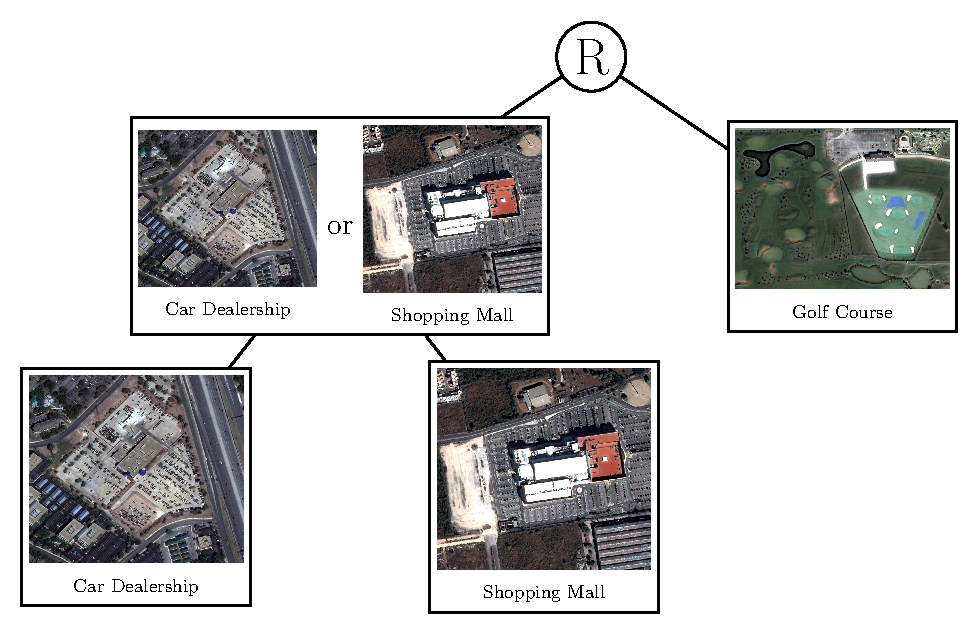
\includegraphics[width=\linewidth]{images/example-hc.pdf}
    \caption[Example Hierarchical Classifier]{This depicts an HC with three
    labels where the meta-classes have already been inferred and now the model
    has to be fit to the data appropriate for the given parent node.}
    \label{fig:example-hc}
\end{figure}

In Figure \ref{fig:example-hc}, there are two parent nodes in the graph: the
root node denoted with an ``R'' and the node which depicts the meta-class
containing the car dealership and shopping mall labels. The simplest way to
train an HC, and technique which is proposed in \cite{yan2015hd},
\cite{bengio2010label}, and \cite{aly2005survey}, and a variety of other authors
who have utilized HCs in their research is to train each classifier in the tree
individually. What this means for the example HC shown in Figure
\ref{fig:example-hc} is that there are two classifiers which need to be fit to
data: $f_1$ and $f_2$. In Figure \ref{fig:hc-w-classifiers} we have circled the
nodes which are contained in each of these classifiers
\begin{figure}
    \centering
    \begin{subfigure}{.49\linewidth}
        \centering
        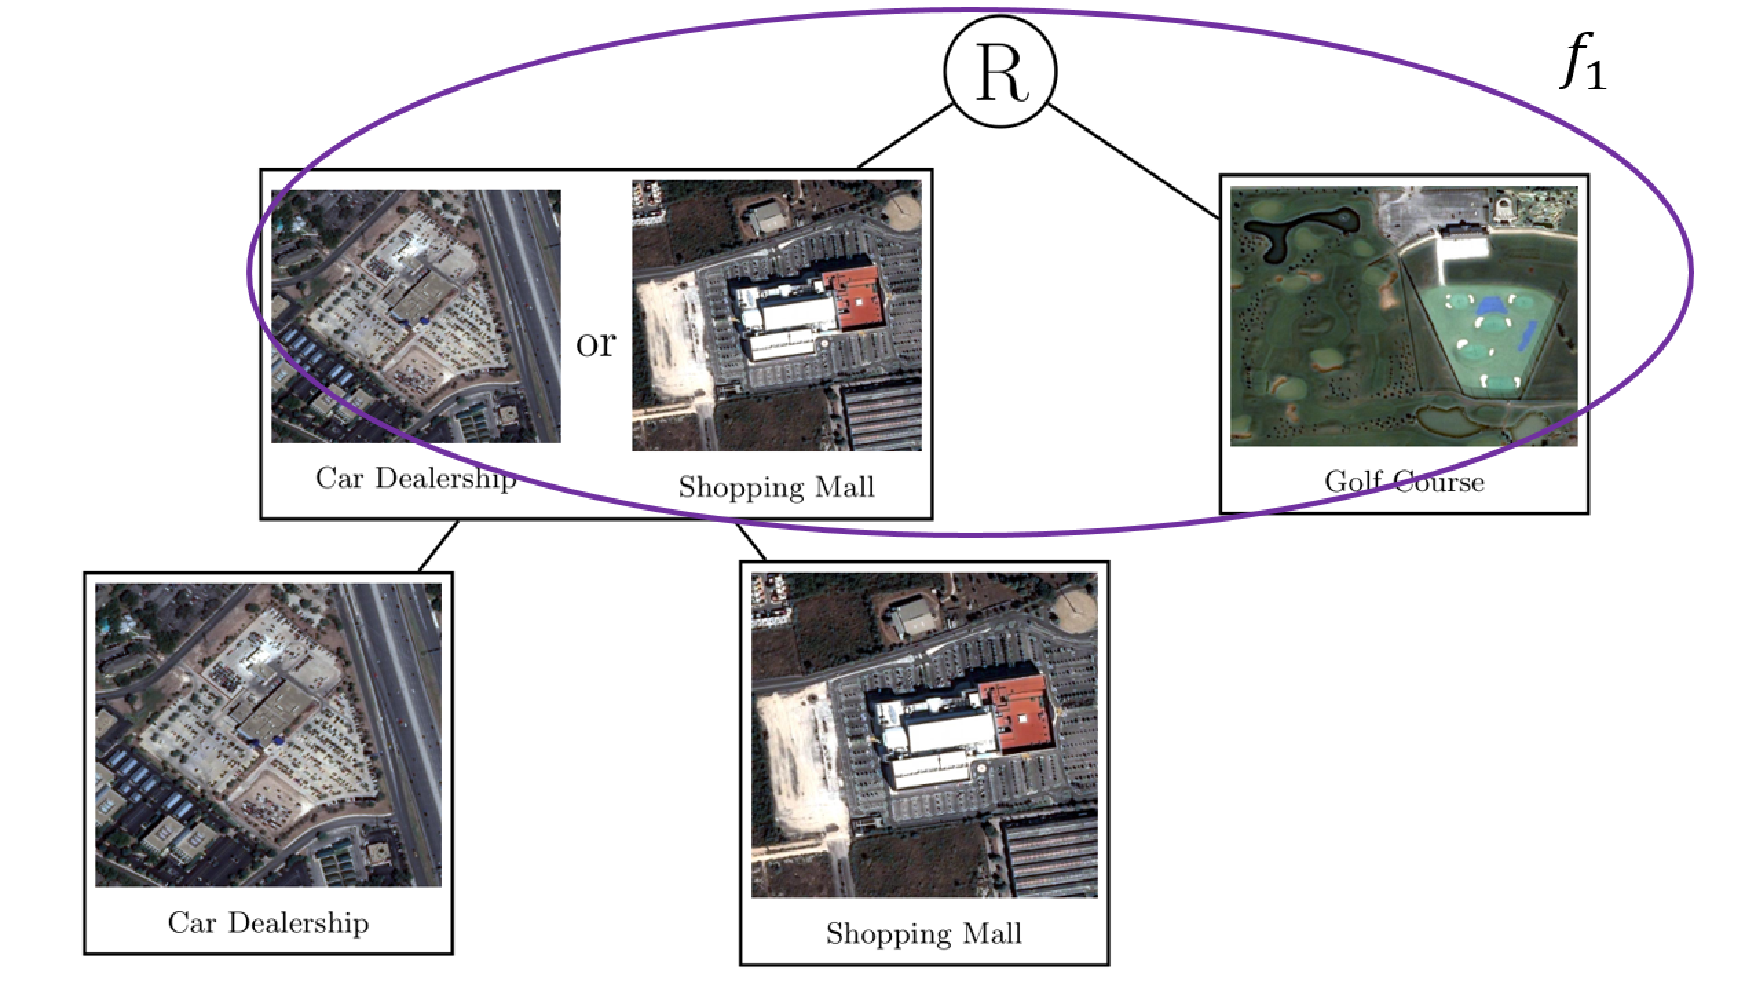
\includegraphics[width=\linewidth]{images/ex-hc1.pdf}
        \caption{$f_1$ HC Estimator}
    \end{subfigure}
    \begin{subfigure}{.49\linewidth}
        \centering
        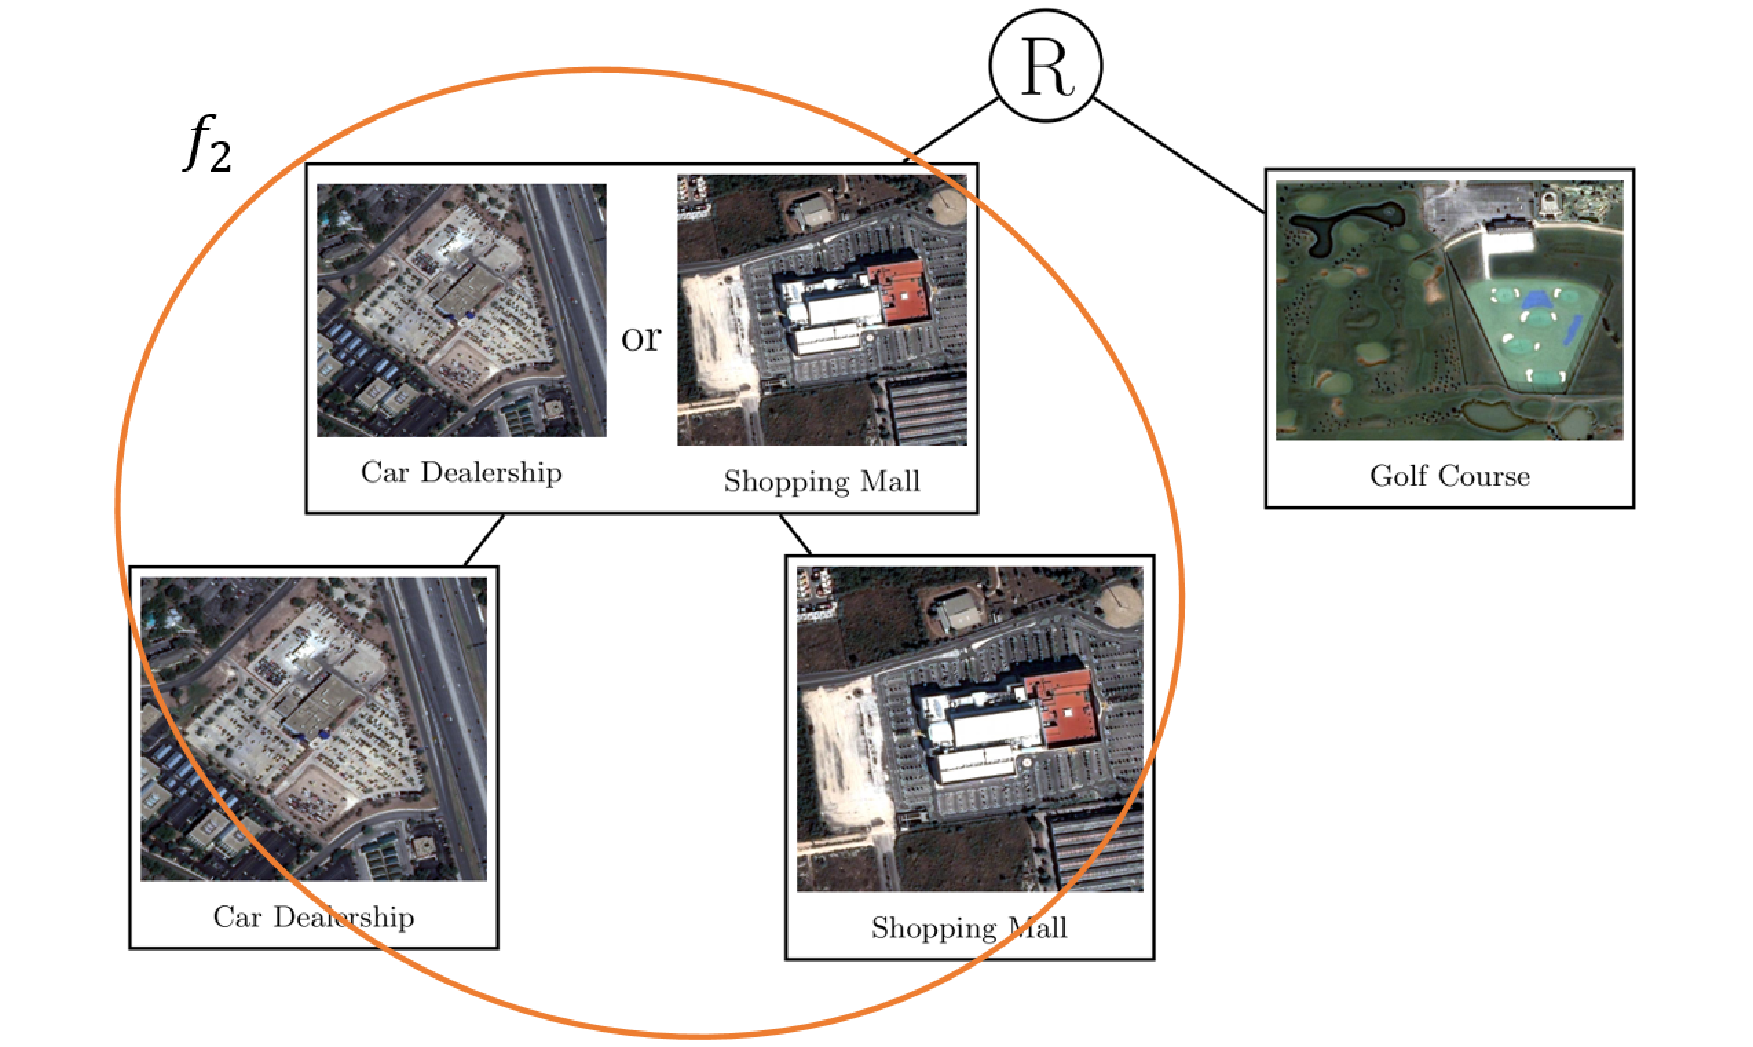
\includegraphics[width=\linewidth]{images/ex-hc2.pdf}
        \caption{$f_2$ HC Estimator}
    \end{subfigure}
    \caption[Example Hierarchical Classifier with Estimator Delineation]{This
    depicts the two classifiers which comprise this particular HC. The
    classifier $f_1$ distinguishes the two meta-classes and the estimator $f_2$
    separate the elements the car dealership and shopping mall label grouping.}
    \label{fig:hc-w-classifiers}
\end{figure}

In general, for any HC, algorithm will fit a classifier which corresponds to the
labels belonging to the parent node in the graph. Thus $f_1$ in Figure
\ref{fig:hc-w-classifiers} denotes that the estimator will predict whether the
sample contains a golf course or is an element in the meta-class, and $f_2$ will
predict to which label the sample belongs in the car dealership, shopping mall
label group. The classifiers $f_1$ and $f_2$ can be trained separately because
they do not share memory; $f_1$ gets the data $\mathcal{D}^1 = (\mathbf{X},
\mathbf{y}^R)$ where $\mathbf{y}^R$ denotes a target vector which has been
re-mapped to the meta-class labels. For example, if car dealership was
represented by label zero, shopping mall by one, and golf course as two, and
$\mathbf{y} = (0, 1, 2)$ then $\mathbf{y}^R = (0, 0, 1)$. Similarly, the second
classifier, $f_2$ gets the training data $\mathcal{D}^2 =
(\mathbf{X}^{\mathcal{M}_1}, \mathbf{y}^{\mathcal{M}_1}$ where $\mathcal{M}_1$
denotes the first inferred meta-class in the data and thus the data matrix and
target vector is solely comprised of elements, in the case of Figure
\ref{fig:example-hc} belonging to the car dealership and shopping mall labels.
Clearly, $f_1$ and $f_2$ do no share any data and thus it is legitimate to train
them separately. Moreover, by this construction, this also allows us to train
$f_1$ and $f_2$ in parallel because this is what as known as an ``embarrassingly
parallel'' problem or one which the tasks (i.e., training $f_1$ and $f_2$) can
be easily separated \cite{herlihy2012art}.

\subsection{Unique Features}
In addition to training $f_1$ and $f_2$ separately, an observation one can make
between $f_1$ and $f_2$ is that the things which separate a golf course from the
other two labels are not the same ones which distinguish the shopping mall from
the car dealership. To make the first classification with $f_1$, one simple
feature (although we do not use this, we use features inferred from CNNs, this
is done purely for explanatory purposes) might be whether a large portion of the
picture is green. If it is, then the sample is likely a golf course, but if it
not it probably falls into the other meta-class. For $f_2$, however, the
distinction between the labels is more subtle. Typically shopping malls are
larger and may have fewer things trying to grab the attention of the customer
(car dealerships can sometimes have ``wacky waving inflatable arm flailing tube
men'' \cite{wacky_wavy} and other things to capture a customer's attention). A
reasonable inference though from these observations is that $f_1$ and $f_2$
should be given different features since what might be informative for $f_1$ may
not be for $f_2$ (e.g., whether there is green in a picture).

This idea has recently been recognized in the HC literature primarily when
authors utilized CNNs for their HCs \cite{yan2015hd} \cite{wang2018learning}.
Convolutional networks are implemented because as discussed in Chapter 2, their
algorithm implicitly infers new features and thus if $f_1$ and $f_2$ were both
CNNs, there is a high chance that the models would develop different filters for
their respective task. However, there are situations when employing a CNN is an
inappropriate model for the data or is too computationally expensive, but we
still want to be able to use this hierarchical framework.

Thus, in our research we propose to use methods which can infer features
relevant for the given classifier that can be applied for any model -- not just
CNNs. To meet this condition, an algorithm must be able to meet the following
conditions:
\begin{enumerate}
    \item Be computationally tractable
    \item Infer features which utilize the labels
\end{enumerate}
The more important of these two requirements is the second one -- that the
features which are inferred for the given classifier utilize the labels. This
point is brought up because there are a number of dimensionality reduction
algorithms which we will infer new features for a given classifier. For example,
principal component analysis (PCA) would generate new features from $\mathbf{X}$
and will typically do so in a computationally tractable manner. Nevertheless,
the algorithm does not employ any information about the labels, $\mathbf{y}$,
and so they are not an appropriate feature generation technique
\cite{jolliffe2011principal}.

The algorithm which we utilize in our experiments is linear discriminant
analysis (LDA). At a high level the objective of multi-class LDA is to find a
projection matrix, $\mathbf{W} \in \mathbb{R}^{p \times d}$, which transforms
the data from $p$-dimensional space to $d$-dimensional space where $d \leq
(C-1)$. This implicitly assumes that $p > d$. Formally, the algorithm tries to
find projection which maximizes the ratio of total between-class spread over
total within-class spread. The intuition behind this approach is that a good
projection should have a large separation between the class labels
(between-class spread) and a compact representation of the label itself
(within-class spread). Within-class is defined as
\begin{equation}
    \mathbf{S}_j = \sum_{\mathbf{x}_i \in \mathcal{C}_j} (\mathbf{x}_i -
    \boldsymbol{\mu}_j)(\mathbf{x}_i - \boldsymbol{\mu}_j)^T
\end{equation}
where $\boldsymbol{\mu}_j = \frac{1}{N_j} \sum_{\mathbf{x}_i \in \mathcal{C}_j}
\mathbf{x}_i$. Between class spread is defined as
\begin{equation}
    \mathbf{S}_B = \sum_{j=1}^C N_j (\boldsymbol{\mu}_j -
    \boldsymbol{\mu})(\boldsymbol{\mu}_j - \boldsymbol{\mu})^T
\end{equation}
where $\boldsymbol{\mu} = \frac{1}{N} \sum_i \mathbf{x}_i$. Using those
matrices, the projected within and between-class spread is defined as
\begin{equation}
    \mathbf{S}_B^\prime = \mathbf{W}^T \mathbf{S}_B \mathbf{W}
\end{equation}
and
\begin{equation}
    \mathbf{S}_W^\prime = \mathbf{W}^T \mathbf{S}_W \mathbf{W}
\end{equation}
where $\mathbf{S}_W = \sum_j \mathbf{S}_j.$ The solution to the LDA problem is thus
\begin{equation}
    \label{eq:lda}
    \mathbf{W}^* = \argmax \quad \frac{\left| \mathbf{S}_B^\prime \right|}
    {\left| \mathbf{S}_W^\prime \right|}.
\end{equation}
Problem (\ref{eq:lda}) is solved as generalized eigenvector problem
\cite{mika1999fisher}.

Returning to the two criteria we proposed, we stated that any algorithm which
generates new features for a particular node must be computationally tractable
and must use the labels to help infer new features. An open-source
implementation of this algorithm in Scikit-learn uses singular value
decomposition to solve (\ref{eq:lda}) which has a number of fast algorithms such
as \cite{halko2011finding}. Moreover, since the means of each class,
$\boldsymbol{\mu}_j$ are used to compute the within-class spread, the labels are
also utilized to infer the new features.

One reasonable critique of this approach is that LDA forces us to find a linear
representation of the data which may not be appropriate. This is fair, but the
reason we selected LDA is because it is freely available on open-source software
and existing non-linear versions of the algorithm have difficulty scaling to
larger problems (one of our data sets has $200,000$ samples) and more
importantly there was not an existing code that could be easily integrated
\cite{park2005nonlinear}. However, in general, as long as the feature extraction
meets the two criteria that were listed previously, it is a valid approach.

\subsection{Routing Problem}
\label{routing-problem}
Thus far we have described how we train a hierarchical classifier and how we can
boost its performance by giving features relevant to the specific classifier.
The last component of utilizing an HC for a classification problem is to
generate test sample predictions using the model.

Suppose that we had some test sample $\mathbf{x}^T$ and we wanted to determine
the most likely label to which $\mathbf{x}^T$ belongs in the HC depicted in
Figure \ref{fig:example-hc}. The simplest way of approach this problem is to
start at the root of the tree generate predictions for each level and select the
label which gives the highest posterior probability. For this specific case,
suppose the posterior probability generated from $f_1$ is the vector
$\hat{\mathbf{y}} = (0.51, 0.49)$. Using the previously mentioned strategy our
algorithm would then proceed to make a prediction using $f_2$. Since this is the
terminating node in the tree, the label with the largest posterior probability
would be the final prediction made by the model for sample $\mathbf{x}^T$. But
what if the prediction the model made at the root was wrong? Because the golf
course had a lower probability, the algorithm eliminated it as a possibility.
However, if the true label was actually the golf course, by removing it as
possibility by using the schema of always going down the tree in the direction
of the largest posterior probability, it is possible that the true sample could
be lost because the algorithm has disregarded it as a possibility. This is known
as the ``routing problem'' because if the algorithm chooses the wrong ``route''
in the HC graph, then using the policy of always selecting the largest value can
lead to situations where the true label is lost. This problem is particularly
pernicious when posterior predictions yield similar values like demonstrated in
the example above.

Most of the time when using HCs, this problem is simply accepted as an implicit
downside of the algorithm. Specifically HCs were originally developed to
decrease test time performance such as with \cite{vural2004hierarchical} and
\cite{bengio2010label}; an alternative approach in which one gets posterior
predictions from all of the labels was out of the question because that would
defeat their entire purpose of designing the algorithm.

However, our goal by utilizing an HC is \textit{not} to decrease the time to
make test set predictions, but rather to perform better in situations when there
are similar labels. Thus one way to get around this issue is to ignore it all
together. Specifically, instead of just going with the highest posterior
probability, why not get the posterior predictions from every classifier in the
Hc and then combine them using the law of total probability (LOTP). The HCs we
propose in our research all have two layers, thus the algorithm calculates:
\begin{equation}
    \label{eq:routing}
    \P\left(y_i = j \mid \mathbf{x}_i \right) = \sum_{l=1}^L \P\left(y_i \in
    \mathbf{Z}_l \mid \mathbf{x}_i\right) \P\left(y_i = j \mid \mathbf{x}_i,
    y_i \in \mathbf{Z}_l\right) \quad \forall j
\end{equation}
and then the highest value of $P(y_i = j | \mathbf{x}_i)$ is selected as the
final test sample prediction. The advantage of using (\ref{eq:routing}) over the
standard arg-max approach is that the algorithm will never eliminate a label as
a possibility and thus we have effectively skirted the ``routing problem.''

\section{Evaluation Metrics}
Finally, in addition to inferring reasonable meta-classes and training the HC,
we need a way to evaluate how the classifier did both at the leaf level of
making fine-grained predictions and at higher levels of whether it can
distinguish meta-classes from one another. In this section we will introduce the
leaf and node-level metrics which are utilized extensively to evaluate the HC
algorithm in Chapters 4 and 5.

\subsection{Leaf-Level Metrics}
One of the most common ways of evaluating a classifier is to determine its
classification accuracy. The HC, as mentioned in Section \ref{routing-problem}
will generate a posterior distribution: $p(y | \mathbf{x}_i)$. The way the
algorithm then makes the final classification is by selecting the class with the
largest probability value -- this is denoted by the variable, $\hat{y}_i$. To
determine if this prediction was correct, the algorithm checks if $\hat{y}_i$
equals the true label, $y_i$. Thus classification accuracy -- or what we will be
referring as ``Leaf Top 1'' in Chapters 4 and 5 is defined as
\begin{equation}
    \text{LT}_1 = \frac{\sum_{i=1}^n \mathbbm{1}(y_i = \hat{y}_i)}{n}.
\end{equation}
We call the standard classification accuracy ``Leaf Top 1'' because it
corresponds to the top prediction made at the leaf level of the HC tree.
Similarly a generalization of $\text{LT}_1$ is ``Leaf Top $k$.'' For this
schema, we get the labels that correspond to the top $k$ posterior values from
$p(y | \mathbf{x}_i)$ and check if the true label, $y_i$ is an element of this
set. We denote the set of the top $k$ largest values of $p(y | \mathbf{x})$ as
\begin{equation*}
    T_k = \underset{p^\prime \subset p, \ |p| = k}{\argmax} \quad \sum_{j=1}^C
    p(y = j | \mathbf{x}).
\end{equation*}
Using this set, ``Leaf Top $k$'' is then defined as
\begin{equation}
    \text{LT}_k = \frac{\sum_i \mathbbm{1}(y_i \in T_k)}{n}.
\end{equation}
In our experiments we typically use Leaf Top 3, but this of course can be
adjusted to scale to the label size in the data.

\subsection{Node-Level Metrics}
Another set of metrics that an analyst might be interested in is the performance
of the HC at the node level (i.e., how well does the HC do distinguishing the
meta-classes it has inferred). One of the benchmarks we employ is what we refer
to as a ``flat classifier'' or the standard classifier which predicts all the
labels at once. This metric cannot be applied to it because the notion of
meta-classes does not make sense for that estimator. Thus, this metric -- which
we will refer to as ``Node Top 1'' -- is defined only for HCs.

However, the primary difficulty of developing this metric is that when comparing
two hierarchical classification methods (e.g., the k-means and community
detection based approach) it is not guaranteed that these estimators have the
same number of classes. For example, suppose that the k-means approach found
that ten meta-classes was best and the community detection algorithms inferred
five. If we then used the standard classification approach of seeing if the
predicted label from the given HC matched the true label re-mapped to the
corresponding label groups, we would not be getting an apples-to-apples
comparison between the estimators. Since the community detection approach has
half the number of meta-classes as the k-means approach in this instance, we
would expect that this algorithm would do better because prior probability of
getting it correct is higher.

Recognizing this fact, one might then attempt to normalize by the number of
meta-classes the HC inferred. For example, a computation one would perform to
see how the k-means approach did normalized by the ten meta-classes would be
\begin{equation}
    \label{eq:naive-nt1}
    \frac{\sum_i \mathbbm{1}(\hat{y}_i^R = y_i^R)}{10}.
\end{equation}
The issue this technique is that it implicitly assumes that the labels are
uniformly distributed between the meta-classes. This is not necessarily true and
in extreme cases can give overestimates the HC's performance. For example,
suppose that the HC determine that $L=2$ and one meta-class had $999$ labels and
the contained one. Assuming that the distribution of samples belonging to each
label was approximately similar for this scenario, we would expect that this
classifier at the node level would get this correct in almost all situations.
However, if we then employed (\ref{eq:naive-nt1}) to determine the performance
of the HC, the resulting value would be too optimistic because there is not a
uniform probability of getting it correct at the node level, the correct
normalization value would be $\frac{999}{1000}$. In this scenario, using this
normalization scheme we would in effect be asking the question: how much better
is the true classifier relative to a random classifier. Mathematically this
would correspond to the question:
\begin{equation*}
    \frac{\text{Accuracy of True Classifier}}{\text{Accuracy of Random Classifier}}.
\end{equation*}
Given the limitation mentioned earlier regarding different numbers of
meta-classes between HCs, this is the simplest way we could determine to make an
apples-to-apples comparison between HCs.

However, in the scenario described in the previous paragraph, to get to the
normalization of $\frac{999}{1000}$ -- the accuracy we would expect from a
random classifier -- we had to make the critical assumption that the
distribution of samples in the labels was uniform. This is almost never the
case, and if this assumption did not hold for the data, then the normalization
factor would not be valid. Thus we need a way to calculate the expected accuracy
of a random classifier which does make any parametric assumptions on the data.
To do this we will employ Monte Carlo permutation strategy.

In non-parametric statistics, permutation tests are one of the most common ways
to perform statistical tests using the null hypothesis that the treatment has no
effect \cite{good2013permutation}. However the strict form of the permutation
test assumes that every element of the permutation space it utilized for the
sampling distribution. Even for the smaller data sets, which contain
approximately $10,000$ samples, it is computationally intractable to generate
$10,000!$ permutations of the target vector, $\mathbf{y}$. When facing this
problem, one technique is to utilized Monte Carlo sampling. That is, instead of
utilizing the entire permutation space, generate a large number of permutations
and then use these values to approximate the permutation sampling distribution.
This is how we will compute the expected accuracy of a random classifier.
Namely, we will permute the true label vector a large number of time, compute
how accurate the true predictions are under this permutation, and then calculate
the mean value of the permutation sampling distribution. Using this strategy we
can compute the expected performance of a random classifier without making any
assumptions on the distribution of labels or samples within those classes. Once
we have computed this value, we can then calculate the ratio of how the true HC
predictions do relative to a random classifier. This process is formally
described in Algorithm \ref{alg:nt1-monte-carlo}.
\begin{algorithm}
    \caption{Monte Carlo Permutation HC Comparison}
    \label{alg:nt1-monte-carlo}
    \begin{algorithmic}[1]
        \Procedure{Compare HC}{$\hat{\mathbf{y}}^R$, $\mathbf{y}^R$, $k$}
            \State $T_A \gets \frac{1}{n} \sum_{i=1}^n \left(\hat{y}_i^R = y_i^R
            \right)$
            \State $\mathbf{r} \gets (0, \ldots, 0)$ \Comment{Instantiate a
            vector to hold permutation results}
            \For{$j \in \{1, \ldots, k \}$}
                \State $\mathbf{y}^{R, P} \gets $ Permute $\mathbf{y}^R$
                \State $\mathbf{r}[j] \gets \frac{1}{n} \sum_{i=1}^n
                \mathbbm{1}\left(\hat{y}_i^R = y_i^{R,P}\right)$
            \EndFor
            \State $\bar{R}_A \gets \frac{1}{k} \sum_{j=1}^k \mathbf{r}[j]$
            \State \textbf{return} $\frac{T_A}{\bar{R}_A}$
        \EndProcedure
    \end{algorithmic}
\end{algorithm}

\section{Summary}
In this chapter we described the major methodological contributions that we have
made in the area of hierarchical classification. In particular we covered the
new label grouping methods we have developed, as well as the techniques which we
will employ to train and generate predictions from the HC. Finally we discussed
how we will evaluate the resulting HC at both the standard leaf level as well as
how to compare different HC estimators.

\end{document}
